\section{Simulation and Analysis}
\label{sec:simulation_and_analysis}

In this section, we focus on illustrating the performance and efficiency of the proposed algorithms by looking at a specific observation model and simulating different scenarios.

Consider a two-dimension search space discretized into a world of hexagonal cells.
We use the gray level to show the quantity of entropy in each cell; a darker color indicates higher entropy.
The dimension of a hexagon is determined by the perceptual capabilities of the human.
This way of discretization gives a constant distance from the center of one cell to any of its immediate neighbors, which facilitates modeling the agent observation range.

The observation model of an agent uses the likelihood of detecting an object of interest in cell $ i $, so we have

\begin{equation}
\label{eq:agentObsMdl}
P_{O^{i}_{t}|S^{i}_{t}}(F|T)=
\left\{
\begin{array}{lcl}
    0 & \mbox{if~} i=y^{h}_{t} \\
    1-\gamma^{agent} & \mbox{if~} i \in N^{agent}(y^{h}_{t}) \\
    1 & \mbox{otherwise.}
\end{array}
\right.
\end{equation}

In equation \eqref{eq:agentObsMdl}, $ \gamma^{agent} \in (0,1) $ is the constant of detection for all cells in $ N^{agent}(i) $.
By definition, $ P_{O^{i}_{t}|S^{i}_{t}}(T|T) = 1 - P_{O^{i}_{t}|S^{i}_{t}}(F|T) $.
This equation encodes an observation model where an agent observes perfectly in the cell it visited, while all cell units within the neighborhood have an equivalent discounted by $ 1-\gamma $ uncertainty of the existence of object of interest.
We assume that both the human and the robot adopt same observation model but different parameters of $ \gamma^{agent} $ and $ N^{agent}() $.

\begin{figure} 
  \centering 
  \subfigure[Probability estimation after a human search]{ 
    \label{fig:envHR:a} %% label for first subfigure 
    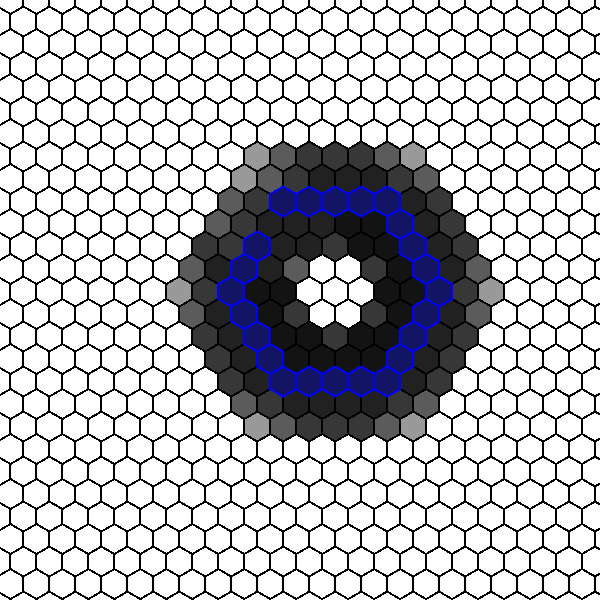
\includegraphics[width=0.2\textwidth]{./images/envH.png}}
  \subfigure[probability estimation after a human search and a robot search]{
    \label{fig:envHR:b} %% label for second subfigure 
    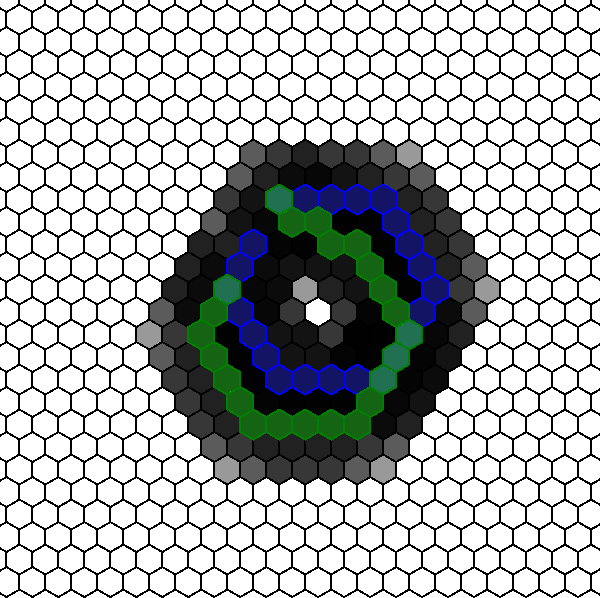
\includegraphics[width=0.2\textwidth]{./images/envHR.png}}
  \subfigure[Problem size and search efficiency as the increase of planning length.]{
    \label{fig:pathPlanningIncrease} %% label for second subfigure 
    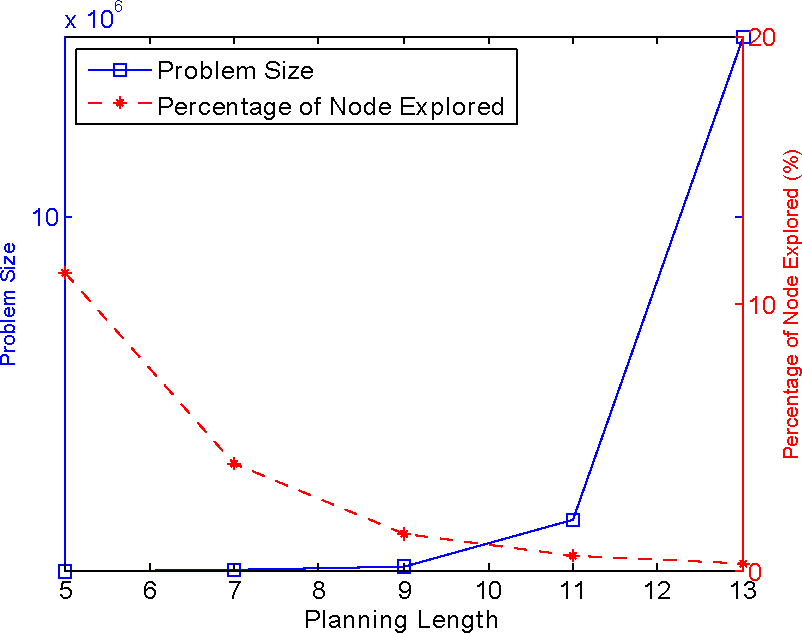
\includegraphics[width=0.32\textwidth]{./images/pathPlanningIncrease.pdf}}  
  \caption{The updates on the probability estimation on where there is a search target.} 
  \label{fig:envHR} %% label for entire figure 
\end{figure}

Figure \ref{fig:envHR} shows the updates on the probability estimation of where there is a search target from observations of agents.
Based on the human path and how the observations of the human update the probability estimation, the robot wingman executes a planned path to maximize the uncertainty reduction on the probability estimation, as in Figure \ref{fig:envHR:b}.

We look at the efficiency and performance of the Algorithm \ref{alg:Anytime} in different types of environments. 
We use below metric to measure the performance and efficiency:
\begin{itemize}
\item \textbf{Problem size: } the number of nodes in the complete expanding tree;
\item \textbf{Optimal total reward: } the maximum total reward in all complete paths;
\item \textbf{Ratio of explored nodes: } the ratio of the number of nodes expanded to the number of the nodes in the complete expanding tree, which indicates the efficiency of Algorithm \ref{alg:Anytime};
\item \textbf{Percentage of optimal at first run: } the ratio of the total reward of the path found at the the first run to the optimal total reward, which indicates how the solution at first run can approximate the optimal;
\item \textbf{Percentage of number of runs reaching the optimal: } the ratio of the number of runs before reaching the optimal to the number of total runs, which indicates the speed of searching optimal.
\end{itemize}

In Figure \ref{fig:pathPlanningIncrease}, we can see that the problem size grows significantly with the planning length increase;
we can see the efficiency of Algorithm \ref{alg:Anytime} as the ratio of the explored nodes decreases with the problem size increase. 

\subsection{Performance and Efficiency}
\label{subsec:performance_and_efficiency}

There are three common types of ways of modeling priori probability estimation on the search space, which are: \emph{uniform}, \emph{random} and \emph{multi-modal}. 
These three are shown in Figure \ref{fig:diffEnv}.  

\begin{figure}[H] 
  \centering
  \subfigure[Uniform.]{ 
    \label{fig:diffEnv:a} %% label for first subfigure 
    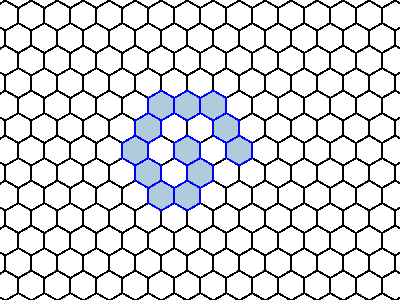
\includegraphics[width=0.3\textwidth]{./images/UniEnv.png}} 
  \subfigure[Random.]{ 
    \label{fig:diffEnv:b} %% label for second subfigure 
    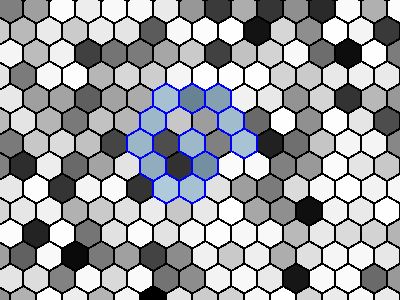
\includegraphics[width=0.3\textwidth]{./images/RndEnv.png}}
  \subfigure[Multi-modal.]{ 
    \label{fig:diffEnv:c} %% label for second subfigure 
    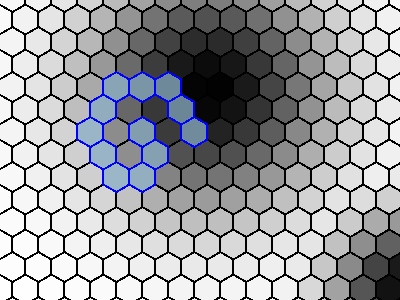
\includegraphics[width=0.3\textwidth]{./images/MMEnv.png}}  
  \subfigure[Performance and efficiency in uniform model.]{ 
    \label{fig:diffEnv:a1} %% label for first subfigure 
    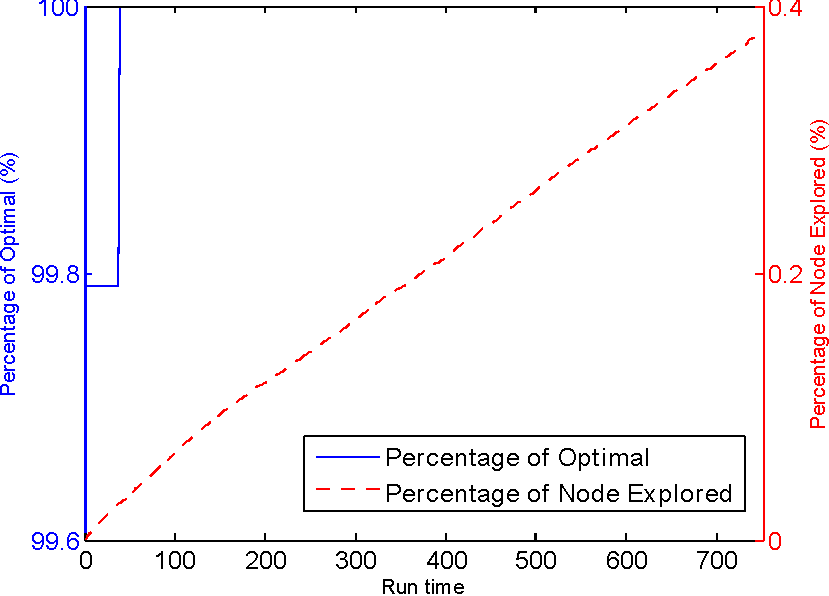
\includegraphics[width=0.3\textwidth]{./images/PM_EnvUni.pdf}}  
  \subfigure[Performance and efficiency in random model.]{ 
    \label{fig:diffEnv:a2} %% label for second subfigure 
    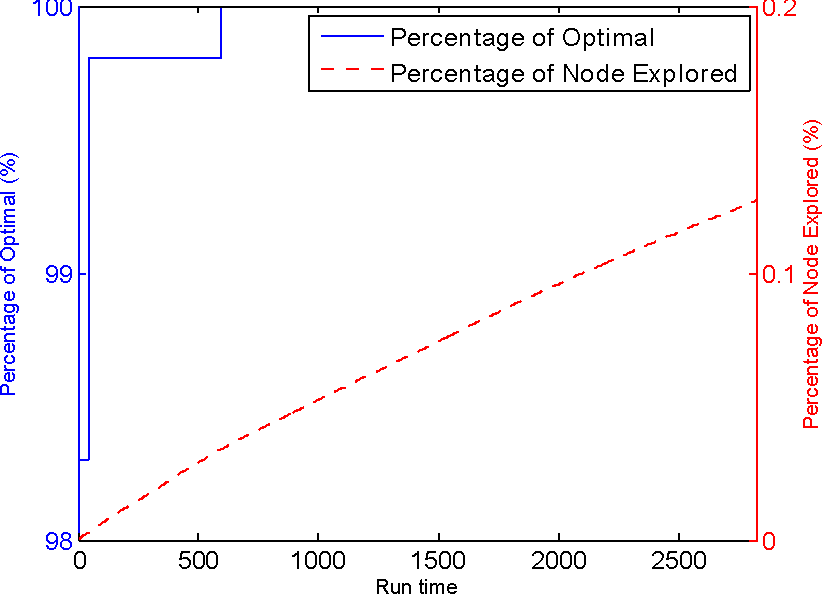
\includegraphics[width=0.3\textwidth]{./images/PM_EnvRnd.pdf}}
  \subfigure[Performance and efficiency in multi-modal model.]{ 
    \label{fig:diffEnv:a3} %% label for second subfigure 
    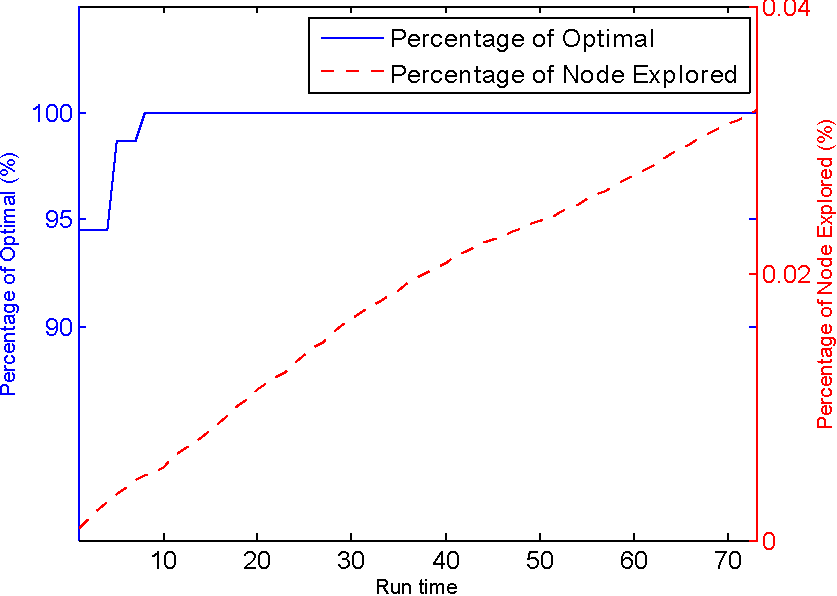
\includegraphics[width=0.3\textwidth]{./images/PM_EnvMM.pdf}}     
  \caption{Different types of priori probability estimation.} 
  \label{fig:diffEnv} %% label for entire figure 
\end{figure}

Usually the estimated maximum future reward by Algorithm \ref{alg:Anytime} has good approximation in uniform model and multi-modal model, due to the smooth gradient of entropy distribution. 
In these two types of environment models, the first several runs of Algorithm \ref{alg:Anytime} can usually find the optimal solution.
We can see that in Figures \ref{fig:diffEnv:a1} and \ref{fig:diffEnv:a3}.
In random model, the estimation on the maximum future reward usually bias from the correct one due to the entropy distribution.
As a result, it takes a longer time to find the optimal solution, which is shown in Figure \ref{fig:diffEnv:a2}
Thus, in the later section, we only look at how Algorithm \ref{alg:Anytime} works with different patterns of human paths in random model.

There are five common patterns of paths executed by a human in a search task, which are:
\emph{line}, \emph{spiral}, \emph{lawn-mower}, \emph{arc} and \emph{loitering}.
Figure \ref{fig:diffHMP} shows examples on these five patterns.
Due to the wingman constraint, different human paths leads to different problem sizes and different ratios of overlap between solution spaces of any two time steps.
Since we focus on the performance comparison, we choose fixed time steps for different patterns, which is $ 11 $ steps shown in Figure \ref{fig:diffHMP}. 

\begin{figure}[H] 
  \centering 
  \subfigure[Line]{ 
    \label{fig:HMP_Line} %% label for first subfigure 
    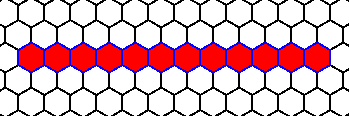
\includegraphics[width=0.2\textwidth]{./images/HMP_Line_Small.png}} 
  \subfigure[Spiral]{ 
    \label{fig:HMP_Sipral} %% label for second subfigure 
    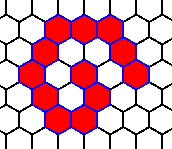
\includegraphics[width=0.14\textwidth]{./images/HMP_Spiral_Small.png}}
  \subfigure[Lawn-mower]{ 
    \label{fig:HMP_LawnMower} %% label for second subfigure 
    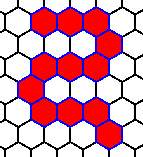
\includegraphics[width=0.14\textwidth]{./images/HMP_LawnMower_Small.png}}  
  \subfigure[Arc]{ 
    \label{fig:HMP_Arc} %% label for first subfigure 
    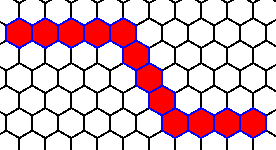
\includegraphics[width=0.2\textwidth]{./images/HMP_Arc_Small.png}} 
  \subfigure[Loitering]{ 
    \label{fig:HMP_Loitering} %% label for second subfigure 
    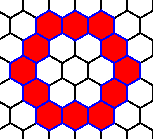
\includegraphics[width=0.14\textwidth]{./images/HMP_Loitering_Small.png}}                
  \caption{Different patterns of human path.} 
  \label{fig:diffHMP} %% label for entire figure 
\end{figure}

Figure \ref{fig:ProbSizeIndiffHMP} shows us that the patterns of spiral and lawn-mower on a human path lead to significantly larger number of expanding nodes in expanding tree structures in comparison with the patterns of line, arc and loitering.
This indicates the difference on the problem sizes in different patterns.
Bigger curvature of a human path generates a larger problem size, because bigger overlap between the flank support regions at two neighboring time steps brings higher connectivities between the nodes in two neighboring partitions in a multi-partite graph.
The problem size grows when the connectivity of the graph topology increases.

\begin{figure}[H] 
  \centering 
  \subfigure[Sizes of solution spaces in different patterns of human paths]{ 
    \label{fig:ProbSizeIndiffHMP} %% label for first subfigure 
    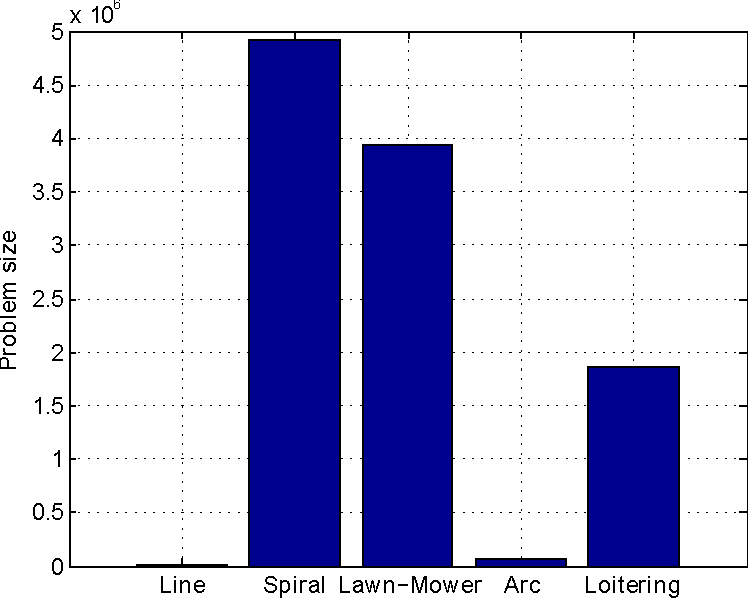
\includegraphics[width=0.45\textwidth]{./images/ProbSizeInDiffHMP.pdf}} 
  \subfigure[Exploration ratios In different patterns of human paths]{ 
    \label{fig:ExoRatioInDiffHMP} %% label for second subfigure 
    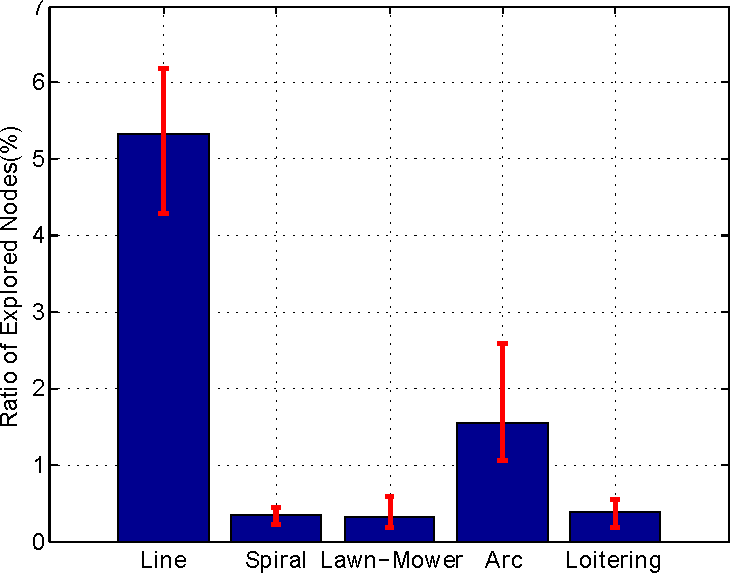
\includegraphics[width=0.45\textwidth]{./images/ExpRatioInDiffHMP.pdf}}
  \subfigure[Percentages of optimal at first iteration in different patterns of human paths]{ 
    \label{fig:InitOptInDiffHMP} %% label for second subfigure 
    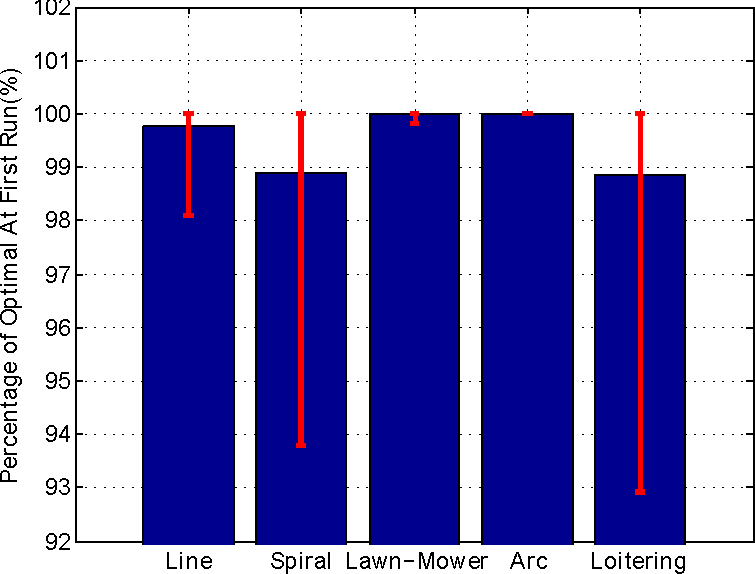
\includegraphics[width=0.45\textwidth]{./images/InitOptInDiffHMP.pdf}}                 
  \caption{Performances in different patterns of human paths} 
  \label{fig:PMdiffHP} %% label for entire figure 
\end{figure}

In contrast to Figure \ref{fig:ProbSizeIndiffHMP}, we can see that in Figure \ref{fig:ExoRatioInDiffHMP} the Algorithm \ref{alg:Anytime} makes significantly better efficiency when the problem size is bigger.
Algorithm \ref{alg:Anytime} also generates a optimal or near-optimal solution at the first runs in different patterns of human paths, which is illustrated in Figure \ref{fig:InitOptInDiffHMP}. 

\subsection{Parameters and Discussion}
\label{subsec:parameters_and_discussion}

The wingman constraint and the observation determine the problem size, the overlaps between flank support coverages and the overlaps between observation coverages.
Here we are going to show how Algorithm \ref{alg:Anytime} adapts to different parameters on problem modeling, which are \emph{flank support range} $ \gamma_{flank} $, \emph{human observation range} $ \gamma^{human}_{obsRange} $  and \emph{robot observation range} $ \gamma^{robot}_{obsRange} $.

\subsubsection{Flank Support Range}
\label{subsubsec:flank_support_range}

\begin{figure}[H] 
  \centering 
  \subfigure[Problem size]{ 
    \label{fig:ProbSizeIndiffWR} %% label for first subfigure 
    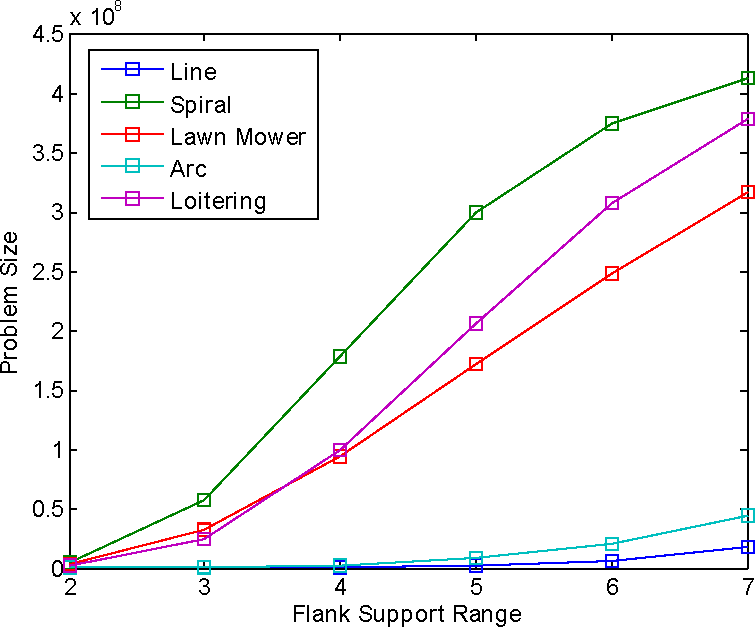
\includegraphics[width=0.45\textwidth]{./images/ProbSizeInDiffWR.pdf}} 
  \subfigure[Optimal total reward.]{ 
      \label{fig:OptScoreIndiffWR} %% label for first subfigure 
      \includegraphics[width=0.45\textwidth]{./images/OptScoreIndiffWR.pdf}}   
  \subfigure[Ratios of explored nodes.]{ 
    \label{fig:ExoRatioInDiffWR} %% label for second subfigure 
    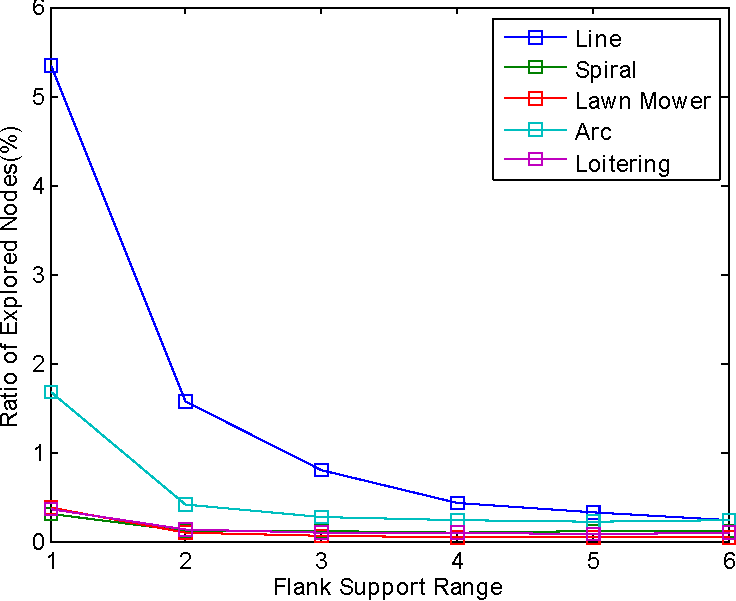
\includegraphics[width=0.45\textwidth]{./images/ExpRatioInDiffWR.pdf}}
  \subfigure[Percentages of optimal at first run.]{ 
    \label{fig:InitOptInDiffWR} %% label for second subfigure 
    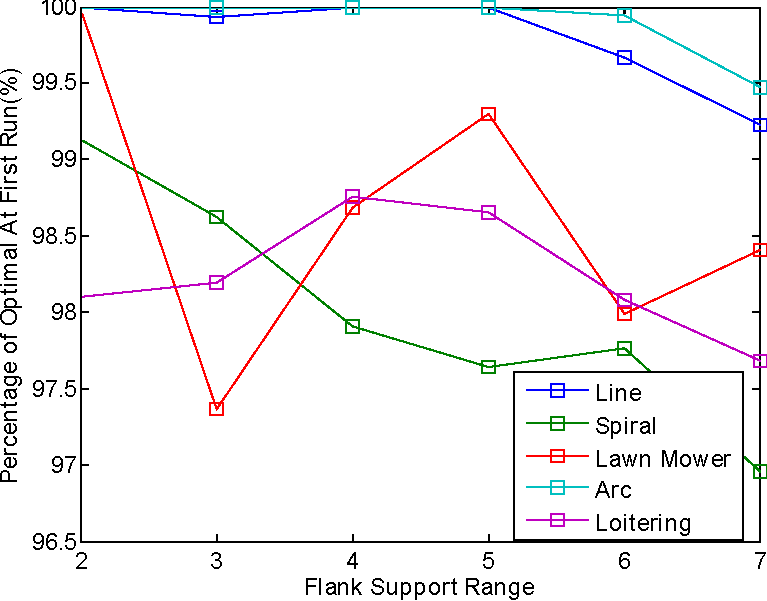
\includegraphics[width=0.45\textwidth]{./images/InitOptInDiffWR.pdf}} 
  \subfigure[Percentages of number of runs reaching the optimal]{ 
    \label{fig:OptHitInDiffWR} %% label for second subfigure 
    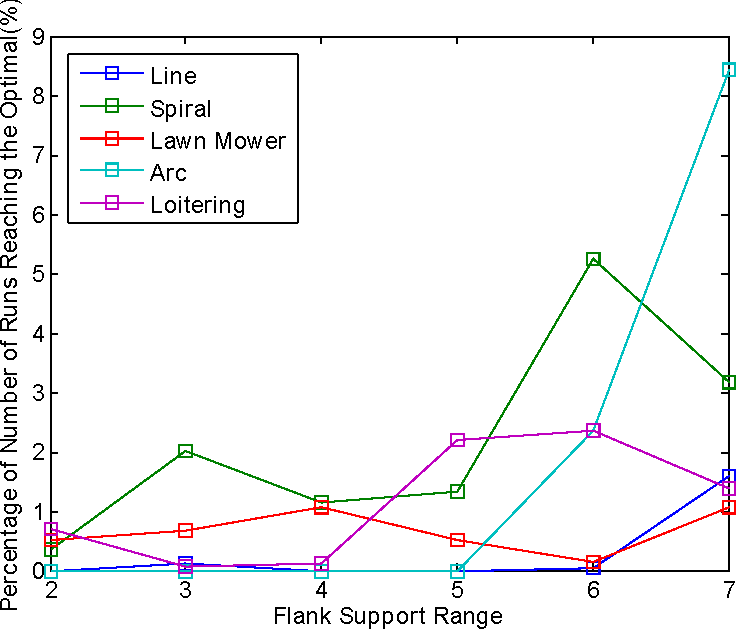
\includegraphics[width=0.45\textwidth]{./images/OptHitInDiffWR.pdf}}                       
  \caption{Different size of the flank support range.} 
  \label{fig:PMdiffWR2} %% label for entire figure 
\end{figure}

When the flank support range is increased, the problem size is also enlarged, as in Figure \ref{fig:ProbSizeIndiffWR}.
The patterns of spiral and lawn-mower show significantly larger growth rates than others. 
The optimal total reward shows a saturation trend with the problem size increase, which is shown in Figure \ref{fig:OptScoreIndiffWR}.
With the increase of problem size, the ratio of nodes explored becomes smaller, which indicates the efficiency improvement.
Figure \ref{fig:ExoRatioInDiffWR} gives an example.
The first run of Algorithm \ref{alg:Anytime} still show good approximate to optimal. 
Relatively, those in the patterns of spiral and lawn-mower are less close to the optimal, which match what are shown in Figure \ref{fig:InitOptInDiffHMP}.
We choose the percentage of the number of runs to find the optimal to measure the speed of optimal search.
Significantly, Algorithm \ref{alg:Anytime} takes longer time to find the optimal solution in the patterns of spiral and lawn-mower, which is illustrated in Figure \ref{fig:PMdiffWR2}.

\subsubsection{Observation Model}
\label{subsubsec:observation_model}

A big human observation range means that the human leave less information for the robot wingman to gather in the vicinity of the regions he visited.
A big robot observation range means that the robot wingman has a stronger capability of information gathering.
The observation model does not change the problem size, thus we focus on the how the performance on optimal search of Algorithm \ref{alg:Anytime} is influenced by these two parameters.

\paragraph{Human Observation Range}

Figure \ref{fig:ExoRatioInDiffHR} illustrates that there are smaller ratio of explored nodes in all the patterns, which indicates the efficiency enhancement.
When the human observation range is large, as most of the entropy will be taken away, the environment for the robot will converge from random to uniform.
Thus, in Figure \ref{fig:InitOptInDiffHR} Algorithm \ref{alg:Anytime} obtains solutions at first run which have good approximations to the optimal in all five patter, which looks like that in Figure \ref{fig:diffEnv:a1}.
We can see that in Figure \ref{fig:OptHitInDiffHR}, the Algorithm \ref{alg:Anytime} shows an increase on the optimal search speed. 
However, when the flank support range surpass some level, the optimal search speed decreases.

\begin{figure}[H] 
  \centering 
  \subfigure[Ratios of explored nodes.]{ 
    \label{fig:ExoRatioInDiffHR} %% label for second subfigure 
    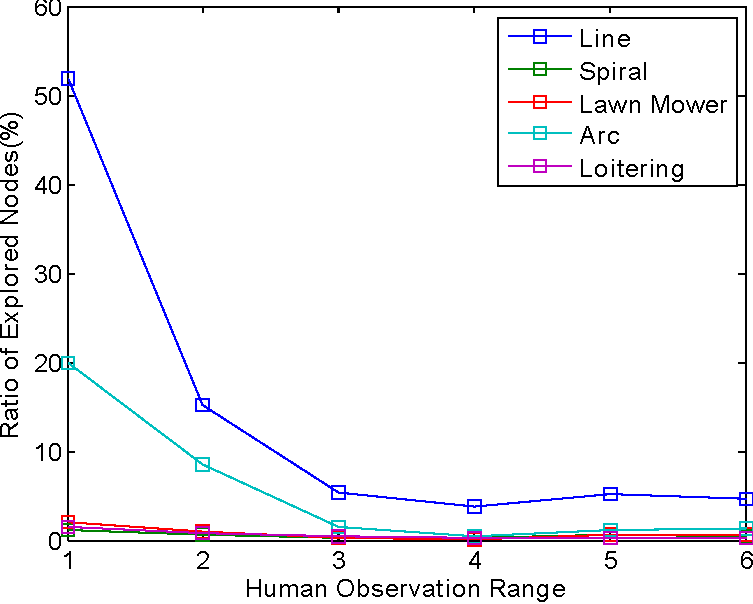
\includegraphics[width=0.45\textwidth]{./images/ExpRatioInDiffHR.pdf}}
  \subfigure[Percentages of optimal at first run.]{ 
    \label{fig:InitOptInDiffHR} %% label for second subfigure 
    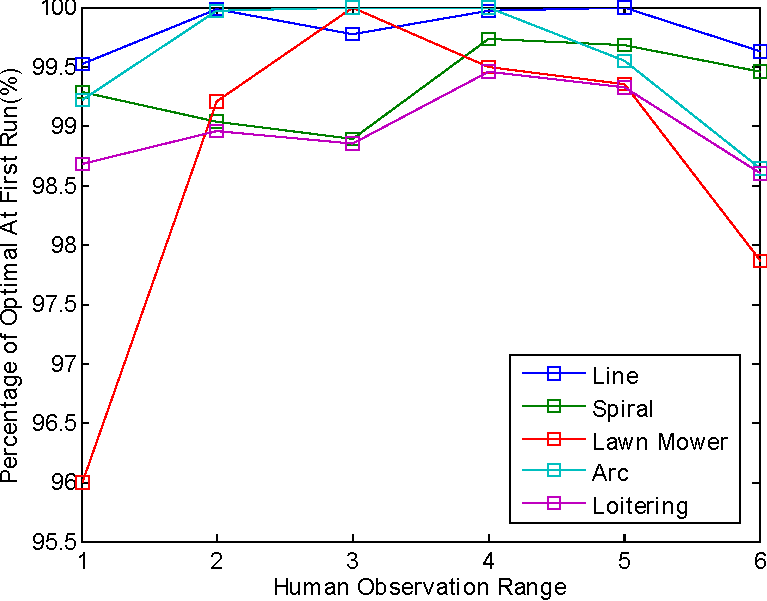
\includegraphics[width=0.45\textwidth]{./images/InitOptInDiffHR.pdf}} 
  \subfigure[Percentages of number of runs reachingthe optimal.]{ 
    \label{fig:OptHitInDiffHR} %% label for second subfigure 
    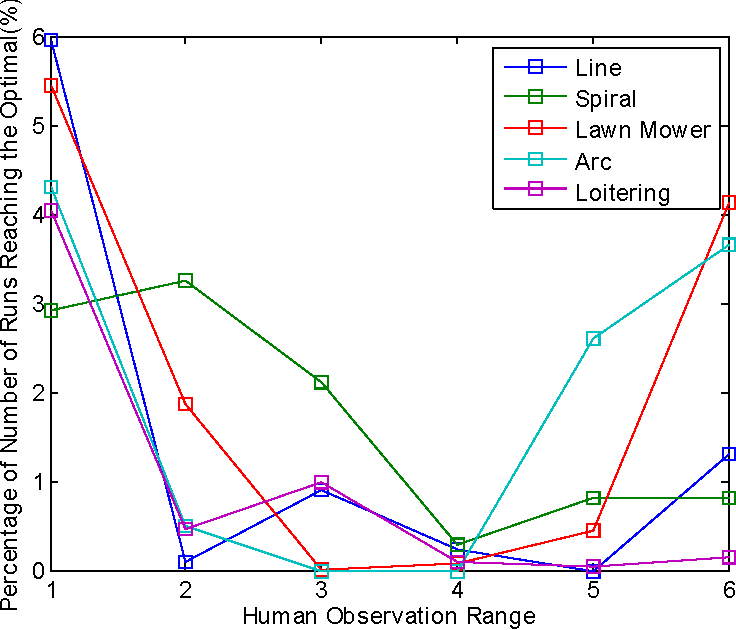
\includegraphics[width=0.45\textwidth]{./images/OptHitInDiffHR.pdf}}                       
  \caption{Different human observation range.} 
  \label{fig:PMdiffHR} %% label for entire figure 
\end{figure}

\paragraph{Robot Observation Range}

When the robot has a larger observation coverage at each time, the overlaps in between are also increased. 
In same problem size, Figure \ref{fig:ExoRatioInDiffRR} shows that Algorithm \ref{alg:Anytime} spends more time to stop in the patterns of line and arc when the robot observation range becomes larger.
However, Algorithm \ref{alg:Anytime} has consistent and good performance on the percentages of optimal at first run in the patterns of line, spiral and arc in Figure \ref{fig:InitOptInDiffRR}. 
The percentages pf number of runs reaching the optimal shows a slow rise in all five patterns, which are shown in Figure \ref{fig:OptHitInDiffRR}.

\begin{figure}[H]
  \centering 
  \subfigure[Ratios of explored nodes.]{ 
    \label{fig:ExoRatioInDiffRR} %% label for second subfigure 
    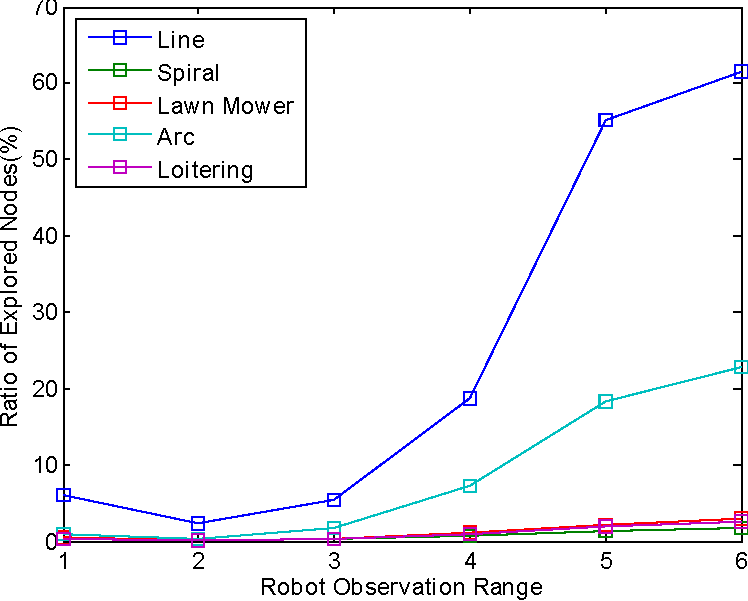
\includegraphics[width=0.45\textwidth]{./images/ExpRatioInDiffRR.pdf}}
  \subfigure[Percentages of optimal at first run.]{ 
    \label{fig:InitOptInDiffRR} %% label for second subfigure 
    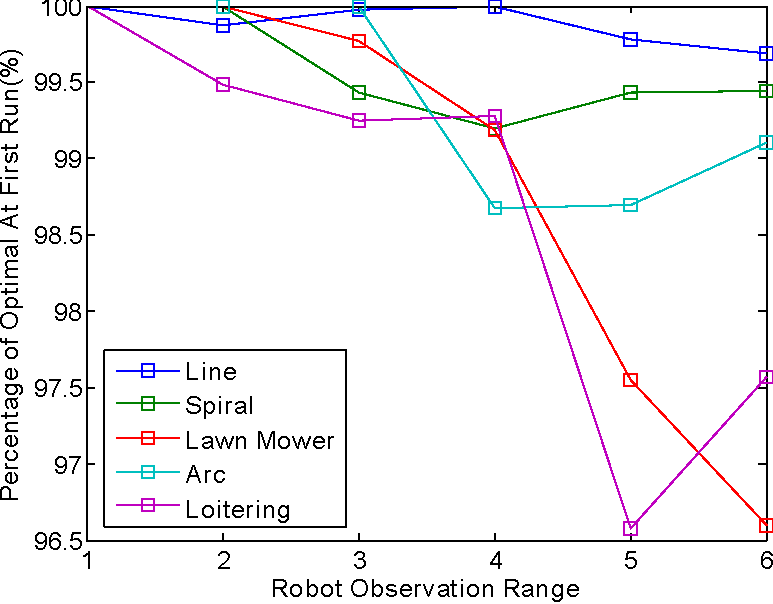
\includegraphics[width=0.45\textwidth]{./images/InitOptInDiffRR.pdf}} 
  \subfigure[Percentages of number of runs reaching the optimal.]{ 
    \label{fig:OptHitInDiffRR} %% label for second subfigure 
    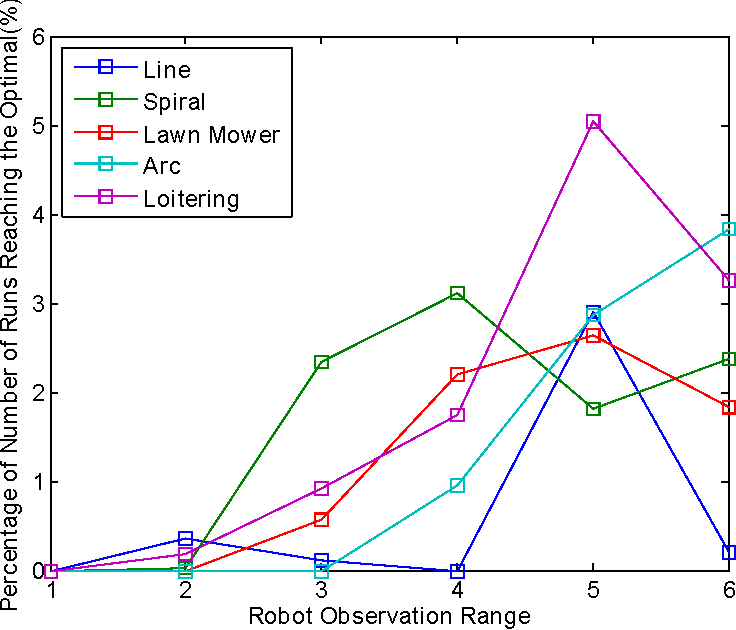
\includegraphics[width=0.45\textwidth]{./images/OptHitInDiffRR.pdf}}                       
  \caption{Different robot observation range.} 
  \label{fig:PMdiffRR} %% label for entire figure 
\end{figure}


\subsubsection{Obstacle}
\label{subsubsec:obstacle}

The existence of obstacles breaks the connectivity between cells in the discretized map.
After mapping to a multi-partite graph, some vertices become terminating and unreachable.
The prune process mentioned in Section \ref{subsec:unfold_solution_space} remove those vertices from the multi-partite graph.
As a result, the problem size is reduced.